\clearpage
\section{Procedure Declaration Concepts} % (fold)
\label{sec:procedure_declaration_concepts}

Chapter \ref{cha:program_creation} \nameref{cha:program_creation} introduced the idea of creating your own Programs as a sequence of instructions, \nameref{sub:statement}s. The instructions in these programs called existing \nameref{sub:procedure}s that performed tasks for the program. The code you wrote sequenced these procedures to produce a desired output.

As you learnt in Chapter \ref{cha:program_creation}, \nameref{sub:procedure}s are designed to perform a single task that can be called when you want that task performed. Using Procedures from Libraries is an important task, but what about the tasks related to the program we are creating? Can we create our own procedures that help us to model the actions we want performed in the code?

The simple answer is \emph{yes}. Yes you can, and should, create your own procedures. These procedures enable you to model the processes related to your program, capturing the individual tasks in the Procedures your create. 

In this Chapter you will learn how to create the following programming \textbf{artefacts}:

\begin{itemize}
  \item \nameref{sub:program_with_procedures_}: Lets you create Procedures in your program's code.
  \item \nameref{sub:proc_decl-procedure_declarations}: Declare the actions the Procedure will perform.
\end{itemize}

\bigskip

You may need to revise the following programming terminology:
\begin{itemize}
  \item \nameref{sub:statement}: An instruction performed in your code.
  \item \nameref{sub:identifier}: The name of an artefact, or the text used to identify something meaningful to the language.
\end{itemize}

This material also requires that you have a good understanding of the following actions:
\begin{itemize}
  \item \nameref{sub:procedure call}: A procedure call is an instruction to run a Procedure.
\end{itemize}

By the end of this material we will have worked through an example where you create a program that writes a small Morse Code message to the Terminal. This program will break the functionality across a number of procedures, making it easy to extend to output other messages. The output of the program is shown in Figure \ref{fig:procedure-decl-morse_calling}.

\begin{figure}[h]
   \centering
   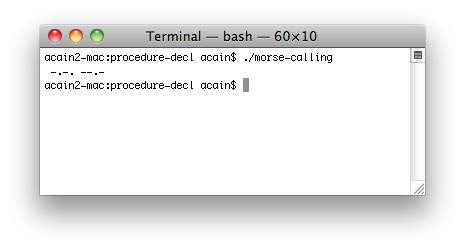
\includegraphics[width=0.9\textwidth]{./topics/procedure-decl/images/MorseCalling} 
   \caption{Morse Calling run in the Terminal}
   \label{fig:procedure-decl-morse_calling}
\end{figure}


\clearpage
\subsection{Program (with Procedures)} % (fold)
\label{sub:program_with_procedures_}

Each Program is a list of instructions (\nameref{sub:statement}s) that command the computer to perform actions. Unfortunately the computer is only able to perform simple actions, meaning that even small programs need many instructions in order to perform their tasks. To help manage these instructions you can group the program's Statements into Procedures, creating Procedures that perform the tasks you need completed in your Program.

\begin{figure}[h]
   \centering
   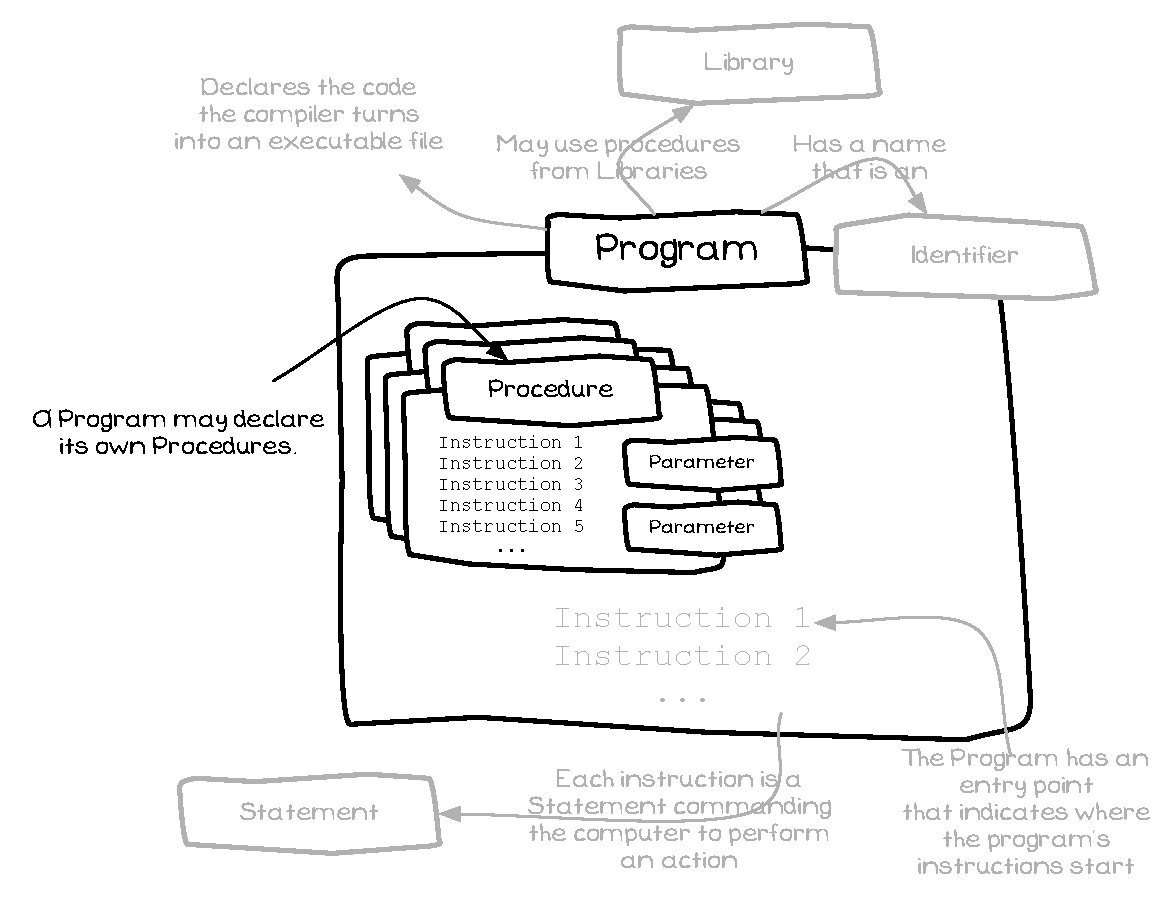
\includegraphics[width=\textwidth]{./topics/procedure-decl/diagrams/ProgramWithProc} 
   \caption{Program with Procedures}
   \label{fig:procedure-decl-program}
\end{figure}

\mynote{
\begin{itemize}
  \item A Program is an \textbf{artefact} that you can \emph{create} in your code.
  \item A Program can contain a number of \nameref{sub:procedure}s.
  \item \nameref{sub:proc_decl-procedure_declarations} allow you to create your own Procedures.
  \item The program's instructions can call the Procedures you create in the program's code.
  \item In C and Pascal the \nameref{sub:proc_decl-procedure_declarations} must appear before they are used in your code.
\end{itemize}
}

% subsection program_with_procedures_ (end)
\clearpage
\subsection{Procedure Declarations} % (fold)
\label{sub:proc_decl-procedure_declarations}

Procedures contain code that define the steps the computer performs when the procedure is called. In your Program you can define your own Procedures, allowing you to divide a Program's tasks into separate Procedures.

\begin{figure}[h]
   \centering
   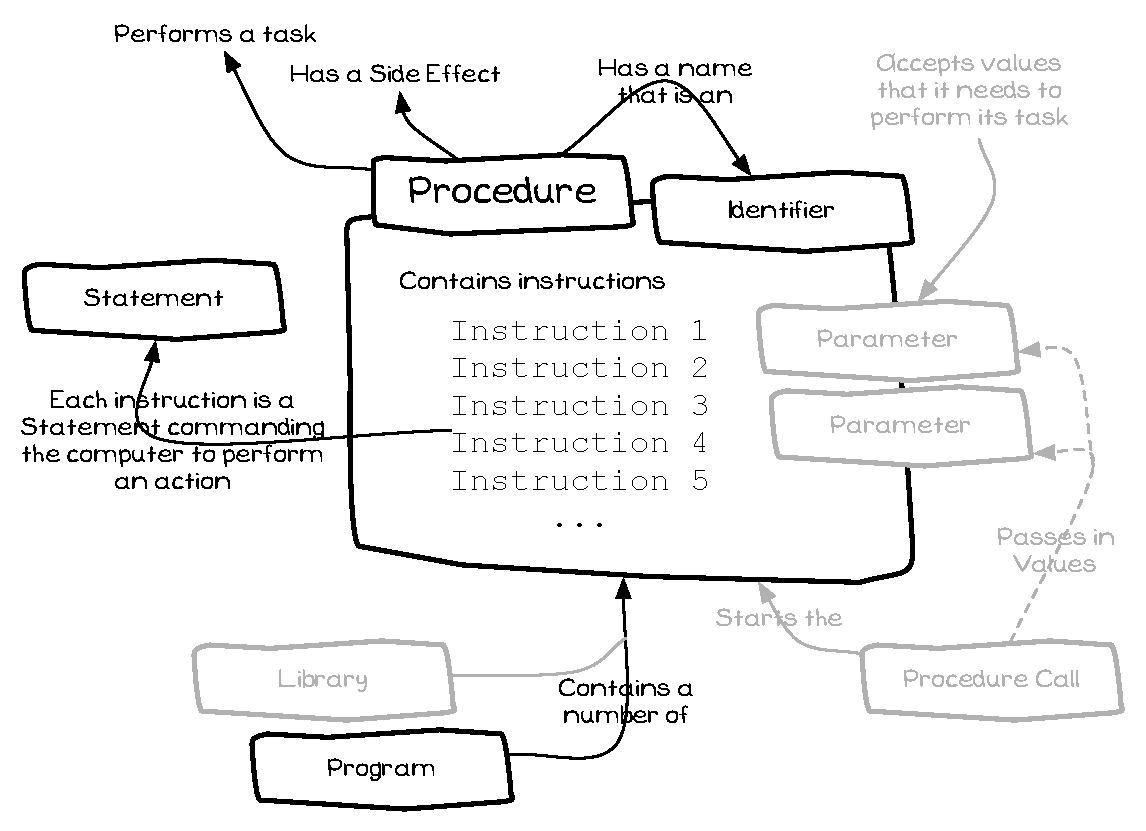
\includegraphics[width=\textwidth]{./topics/procedure-decl/diagrams/ProcedureDeclaration} 
   \caption{Procedure Declaration}
   \label{fig:procedure-decl-procedure-decl}
\end{figure}

\mynote{
\begin{itemize}
  \item A Procedure is an \textbf{artefact} that you can \emph{create} and \emph{use} in your code.
  \item Each Procedure contains code to perform a certain task. When you want the task performed you call the Procedure.
  \item Procedures should have a \textbf{side effect}\footnote{Output to the Terminal is an example of a Side Effect. After calling these procedures the text you wanted to appear was written to the Terminal. These Procedures changed the Terminal.}, meaning that it changes something when it is executed.
  \item The Procedure's declaration defines its \textbf{name}, and the \textbf{steps} it performs.
  \item Each instructions in the Procedure is a \nameref{sec:program-creation-statement}.
  \item The Procedure's \nameref{sec:program-creation-identifier}:
  \begin{itemize}
    \item Is the name used to call the Procedure.
    \item Should be a \textbf{verb} that \textbf{reflects the task} the Procedure performs.
  \end{itemize} 
  \item When the Procedure is called its instructions are executed.
  \item Each Procedure's instructions are isolated from the other code in your Program. When you are working on a Procedure you do not need to know about the internal workings of the other procedures.
\end{itemize}
}

% subsection procedure_declarations (end)

\clearpage
\subsection{Summary} % (fold)
\label{sub:procedure-decl_summary}

This section has introduced you to the idea of creating and using your own Procedures. The concepts related to this are shown in Figure \ref{fig:procedure-decl-summary}. The next section will examine how these concepts can be used to design the Morse Code program.

\begin{figure}[h]
   \centering
   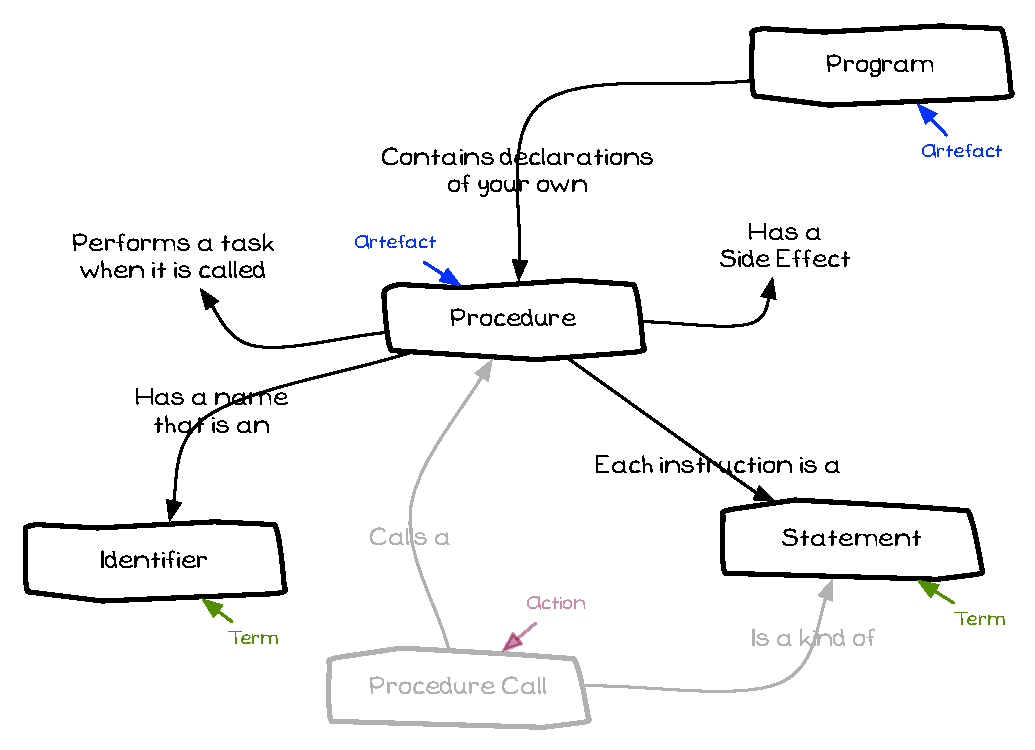
\includegraphics[width=\textwidth]{./topics/procedure-decl/diagrams/Summary} 
   \caption[Chapter Concepts]{Key Concepts introduced in this Chapter}
   \label{fig:procedure-decl-summary}
\end{figure}

\mynote{
\begin{itemize}
  \item \textbf{Artefacts} are things you can \emph{create} and \emph{use}.
  \item \textbf{Terms} are things you need to \emph{understand}.
  \item \textbf{Actions} are things you can \emph{command} the computer to perform.
\end{itemize}
}


% subsection summary (end)


% section procedure_declaration_concepts (end)
